\chapter{DataBase NoSQL}
I database \emph{NoSQL}, che sta per \emph{not only SQL}, sono database non tabellari che archiviano i dati
in maniera completamente differente dai classici relazionali.
Le caratteristiche principali sono la progettazione specifica per carichi elevati e il supporto nativo per la scalabilità
orizzontale, la tolleranza agli errori e la memorizzazione dei dati in modo denormalizzato.
Infatti ogni elemento viene archiviato singolarmente con una chiave univoca, e la coerenza dei dati non viene garantita.
Questa impostazione fornisce un approccio molto piú flessibile alla memorizzazione dei dati rispetto a un database
relazionale, un controllo migliore e una maggiore semplicità nelle applicazioni.

\section{Origine}
A partire dagli anni 2000 si é passati da un modello in cui le persone principali dell'IT erano sistemisti ad un modello
in cui le persone principali sono diventate gli sviluppatori. Tale passaggio ha comportato la nascita di database NoSQL
che sono fortemente orientati agli sviluppatori ed allo sviluppo Agile.
Inoltre i dati si sono trasformati passando dai classici strutturati a quelli non strutturati (di differenti dimensioni,
semi-strutturati, polimorfici...) che non permettono di definire un modello relazionale organico;
così i database NoSQL sono diventati estremamente popolari perché permettono di lavorare principalmente con dati non strutturati anche di enormi
dimensioni.

\section{Perché utilizzare NoSQL}
I database NoSQL sono una soluzione ideale per molte applicazioni moderne, quali dispositivi mobili, Web e videogiochi
che richiedono strutture dati flessibili, scalabili, con prestazioni elevate ed altamente funzionali.
\subsection{Vantaggi}
I principali vantaggi sono:
\begin{itemize}
    \item \textbf{Schemaless}: vengono offerti schemi flessibile che consentono uno sviluppo piú veloce. Quindi é una soluzione ideale
    per i dati semi-strutturati e non strutturati. É possibile arricchire le applicazioni di nuovi dati e informazioni
    senza dover sottostare ad una rigida struttura;
    \item \textbf{Scalabilità}: grazie alla semplicità vi é la possibilità di \emph{scalare in orizzontale} in maniera estremamente
    efficiente. Infatti, si predilige l'utilizzo di cluster con molti nodi distribuiti, rispetto all'utilizzo di server centralizzati.
    Inoltre, vi é la possibilità di aggiungere nodi a caldo in maniera completamente trasparente per l'utente finale;
    \item \textbf{Elevate Prestazioni}: grazie alla mancanza di operazioni di aggregazione dei dati ("join") ed anche grazie
    all'introduzione di semplificazioni, come il mancato supporto delle transazioni ACID, si ha una elevata velocità computazionale;
    \item \textbf{Riduzione dei tempi di sviluppo}: grazie alla definizione di logiche di lettura dati molto piú semplici rispetto a quelle da scrivere con
    database relazionali.
\end{itemize}

\subsection{Limiti}
La semplicità di questi database comporta anche degli svantaggi:
\begin{itemize}
    \item \textbf{Integrità:} mancando i controlli fondamentali sull'integrità dei dati, il compito ricade totalmente sull'applicativo che dialoga con il database;
    \item \textbf{Scrittura}: problema strettamente collegato all'integrità, poiché ogni volta che si deve aggiornare un dato ridondato in piú entitá diventa
    necessario aggiornarlo su tutte le entità in cui é stato duplicato; questo di fatto tende ad aumentare i tempi di sviluppo, anche se le operazioni
    di lettura sono notevolmente semplificate;
    \item \textbf{Standard universale}: ogni database ha il proprio metodo di storing ed accesso ai dati, ne deriva che vi é una mancanza di uno standard
    universale come SQL. Quindi, il passaggio da un database ad un altro puó richiedere alcuni cambi piú o meno radicali da apportare all'applicativo;
    \item \textbf{Espressività}: problema legato ai linguaggi di interrogazione, infatti risulta essere meno espressivo rispetto a SQL nella grande maggioranza dei
    casi, portando ad una maggiore difficoltà di correzione massiva (data fixing), report ed export dei dati.

\end{itemize}

\section{Tassonomia}
I database NoSQL possono essere implementati seguendo diversi approcci a seconda del modello con cui vengono
rappresentati i dati.
A tal proposito, le principali categorie in cui vengono suddivisi sono le seguenti:
\begin{itemize}
    \item \textbf{Document Stores}: la rappresentazione dei dati é affidata a strutture simili ad oggetti, dette \emph{documenti}, ognuno dei
    quali possiede un certo numero di proprietà che rappresentano le informazioni.
    Viene creata una semplice coppia, a una chiave viene assegnato un documento specifico, e in questo documento, il quale puó essere
    formattato in vari modi (XML, JSON, YAML ...), si possono trovare le informazioni.
    La nozione di schema é dinamica, ogni documento puó contenere dei campi diversi.
    Questa flessibilità puó essere particolarmente
    utile per la modellazione dei dati in cui le strutture possono cambiare da un record all'altro, come nei dati polimorfici.
    Inoltre, diventa piú semplice l'evoluzione di un'applicazione durante il suo ciclo di vita, permettendo di aggiungere
    nuovi campi a nuovi record, senza dover modificare i precedenti.

    Tra gli esempi di maggiore interesse vi sono: MongoDB, Azure CosmosDB, Apache CouchDB.
    \begin{figure}[H]
        \begin{center}
            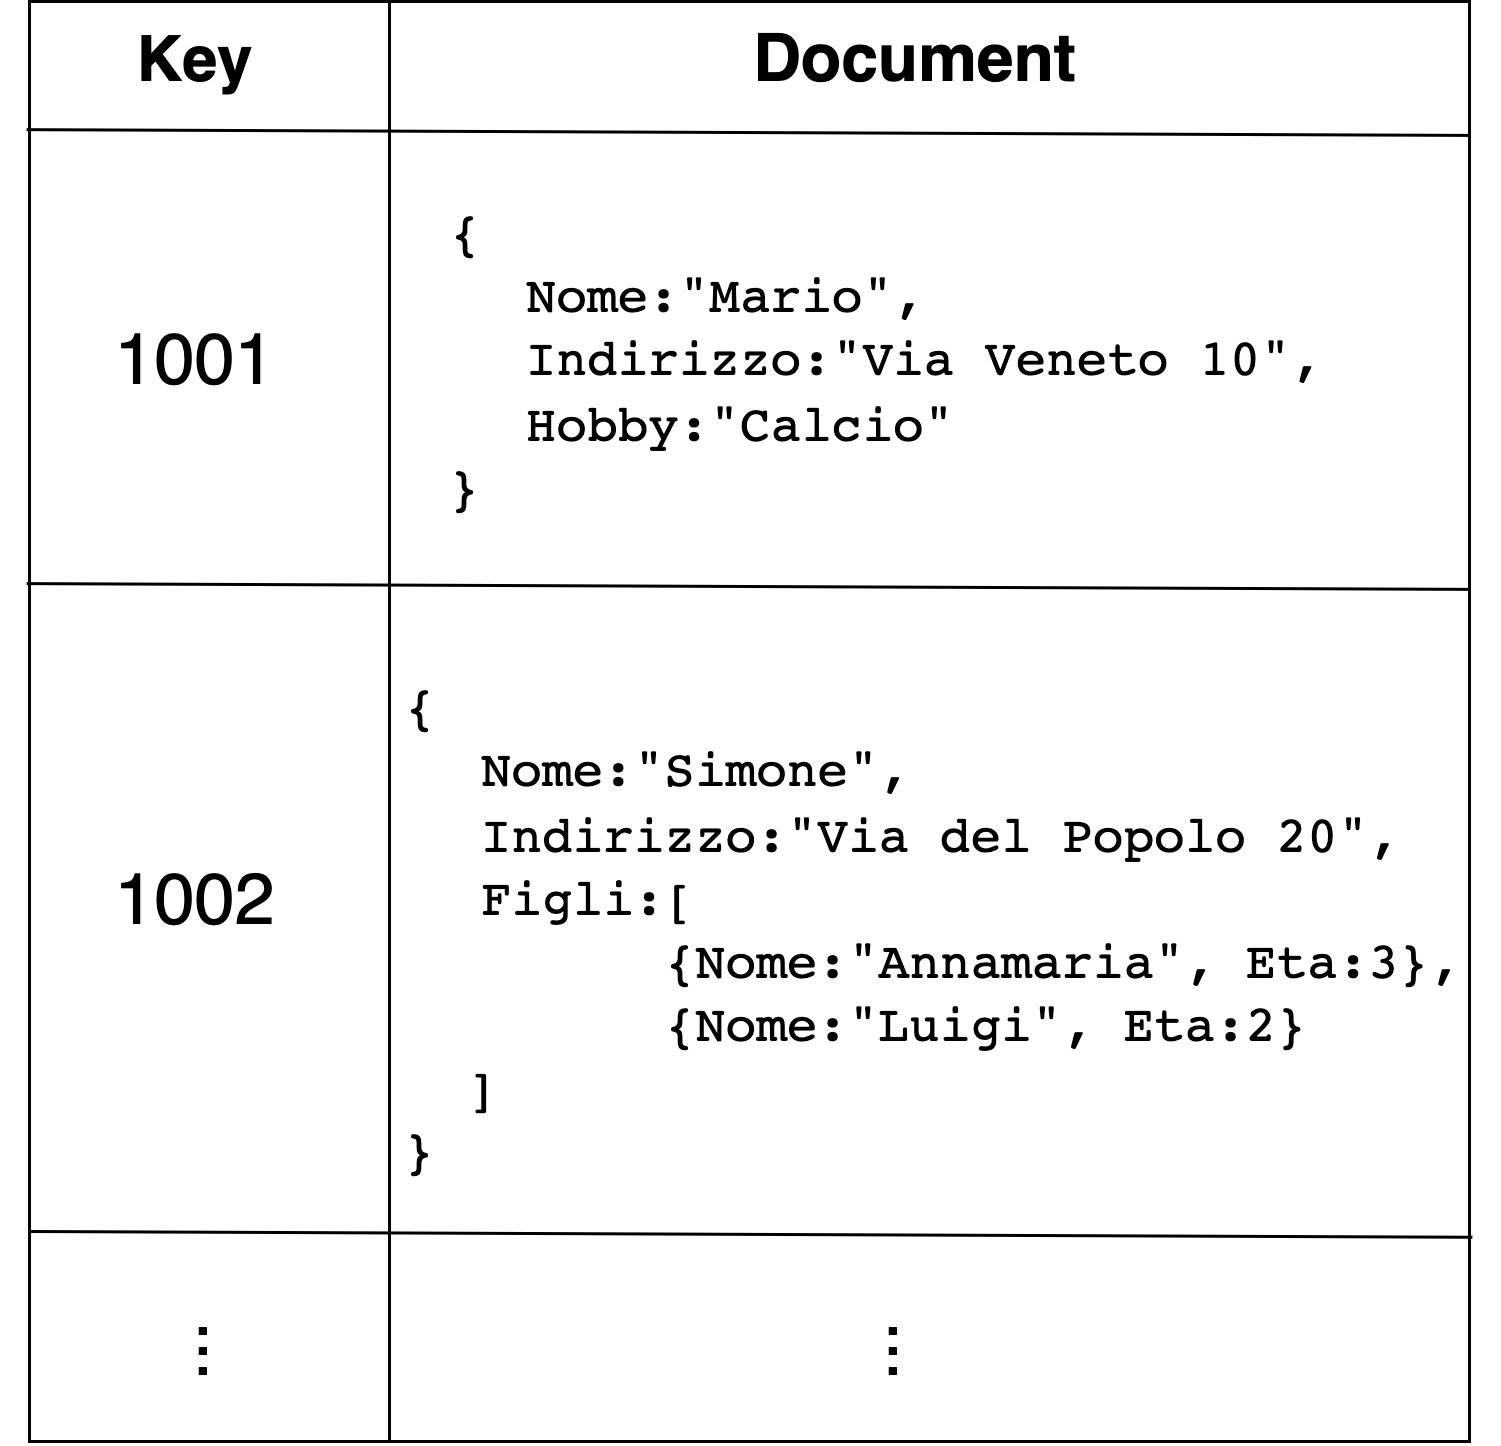
\includegraphics[width=0.7\textwidth]{img/dbDocumentale}
        \end{center}
        \caption{esempio Document Stores database}
    \end{figure}

    \item \textbf{Key-Value Stores}: i dati vengono immagazzinati mediante un semplice metodo chiave-valore. Una chiave rappresenta un identificatore
    univoco. Le chiavi e i valori possono essere qualsiasi cosa, da un oggetto semplice ad articolati oggetti composti.
    (Questo tipologia verrá sviluppato maggiormente nel corso dei prossimi capitoli.)

    Tra gli esempi di maggiore interesse vi sono: \textbf{Redis}, MemCached.
    \item \textbf{Column Family Stores}: i dati vengono archiviati per colonne, anziché per righe come avviene nei database relazionali classici.
    Ogni colonna puó essere memorizzata separatamente, oppure possono essere raccolte per formare dei sottogruppi.
    Infatti, se sono presenti colonne simili, vengono unite in famiglie di colonne, ed ogni famiglia
    viene archiviata separatamente dalle altre su un "file" diverso.
    Questa tipologia di database viene utilizzata quando é necessario un modello di dati di grandi dimensioni.\\
    Estremamente utili per i data warehouse, oppure quando sono necessarie prestazioni elevate o la gestione di query intensive.

    Tra gli esempi di maggiore interesse vi sono: HBase, Cassandra, Vertica.

    \begin{figure}[H]
        \begin{center}
            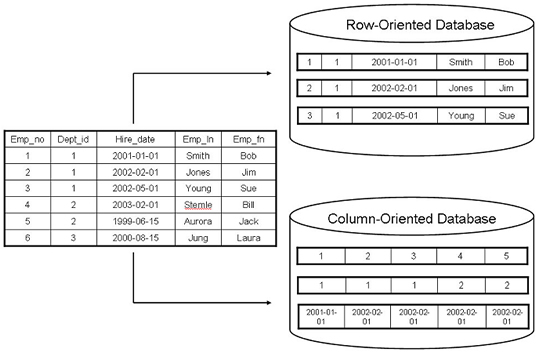
\includegraphics[width=0.9\textwidth]{img/dbColumnOriented}
        \end{center}
    \caption{esempio Column Family Stores database}
    \end{figure}

    \item \textbf{Graph Model}: progettati appositamente per l'archiviazione e la navigazione di relazioni. Le relazioni rivestono un ruolo chiave
    e buona parte del valore di questi database deriva proprio dalla loro presenza. Vengono utilizzati i \emph{nodi} per archiviare le entitá
    di dati e gli \emph{archi} per archiviare le relazioni tra entitá. Le relazioni che un nodo puó avere sono illimitate.
    In questo tipo di database attraversare collegamenti o relazioni é molto veloce perché le relazioni tra i nodi non vengono elaborate al momento
    della query, ma sono giá presenti nel database.\\
    I casi d'uso piú tipici sono i Social Network, motori di raccomandazioni e rilevamento di frodi, ovvero in tutti quegli ambiti dove é
    necessario creare molte relazioni tra dati ed eseguire rapidamente query su di esse.

    Tra gli esempi di maggiore interesse vi sono: Neo4J, Titan.
    \begin{figure}[H]
        \begin{center}
            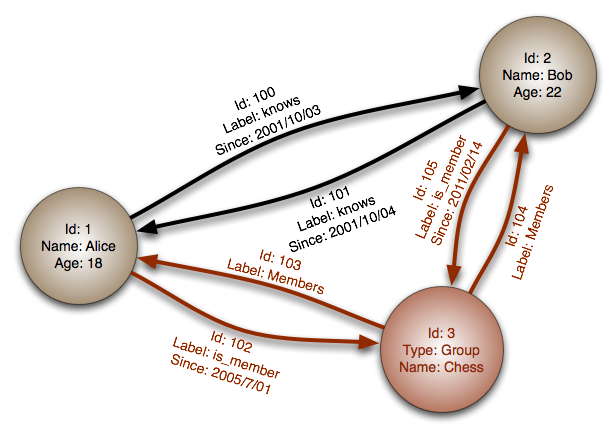
\includegraphics[width=0.8\textwidth]{img/dbGrafo}
        \end{center}
    \caption{esempio Graph Model database}
    \end{figure}
\end{itemize}
